\documentclass[12pt]{eng04457}

\begin{document}

\headertext{Sensors} % texto do cabeçalho das páginas
\ano{\the\year} % ano presente no cabeçalho da capa e copyright ao final
\title{Título do Relatório}
\author{Primeiro Nome, Segundo Nome e Terceiro Nome}
\emails{
    \emailaddress{autor1@email}{iniciais do nome F.L.};
    \emailaddress{autor2@email}{F.L.};
    \emailaddress{autor3@email}{F.L.}}
\datainicio{xx/xx/2015}
\datafinal{xx/xx/2015}

\resumo{Deve conter introdução ao trabalho, método, resultados e conclusões – tudo isso de forma resumida em somente 01 parágrafo. De forma geral e simples deve descrever o que foi feito, porque foi feito e resultado(s) do que foi feito. O Resumo deve ser apresentado apenas no formato de 1 parágrafo e contendo no máximo 300 palavras.}
\resumoeng{Resumo em inglês.}    
\keywords{exemplo; célula de carga; palavras adequadas ao trabalho (no máximo 5 palavras).}

\maketitle 

\section{Introdução}
Texto principal.

Deve conter uma pequena introdução ao assunto tratado com uma pequena revisão bibliográfica (\textbf{com citações de artigos e livros}) e destacar a descrição dos objetivos (principal(is) e o(s) objetivo(s) secundário(s)) do trabalho tratado no referido relatório. No máximo 2 páginas!

\section{Metodologia Experimental}

Texto principal.

Texto principal. Para cada trabalho experimental deve descrever inicialmente o aparato experimental utilizado – com diagrama de blocos resumido do sistema desenvolvido (uma figura bem apresentada ou foto coerente com a descrição dos itens que formam o aparato experimental). Depois abrir em subcapítulos e descrever os principais itens do experimento desenvolvido ou projeto desenvolvido. \textit{\textbf{Este capítulo não deve conter resultados}} e sim a descrição do método/experimento desenvolvido. De forma geral e simples este capítulo deve apresentar “como foi feito” o experimento e evidentemente para isso deve descrever todo e qualquer item utilizado no experimento (cuidado apenas para não tornar o relatório infantil e “sem fundamentação científica” nos experimentos simples principalmente).

Toda e qualquer figura e tabela deve conter a respectiva chamada no texto, por exemplo, A Figura 1 apresenta o diagrama de blocos do experimento desenvolvido para calibrar...etc. A Tabela 1 apresenta os dados....etc. Equações também devem seguir a seguinte formatação (utilizar um bom editor de equações) e as mesmas devem ser numeradas sequencialmente no texto. Por exemplo:

\begin{equation}
    \text{[adicionar uma equação aqui; usar MS Word or MathType equation function]}
\end{equation} 
(retirar os colchetes ao anexar a equação – não esquecer que após anexar a respectiva equação no texto as variáveis da equação devem ser descritas). Por exemplo, a Equação (1) representa a...etc....

\begin{equation}
    V=R \times i
\end{equation}
onde V representa a tensão elétrica [V], R a resistência elétrica [ohm] e i....

Texto principal. Todo e qualquer circuito devem conter a respectiva equação de medição....

Texto principal. Programas desenvolvidos devem apresentar o fluxograma da rotina e a descrição dos principais blocos ou funções desenvolvidas e/ou utilizadas no corpo principal do texto (o restante pode ser colocado em um apêndice no final do relatório – não esquecer de apresentar a respectiva chamada, como por exemplo, a rotina principal do....bláblá.....encontra-se no Apêndice 1. A Figura 2 apresenta o fluxograma representando a rotina para ...... e descrever os principais blocos.

\begin{figure}[H]
    \centering
    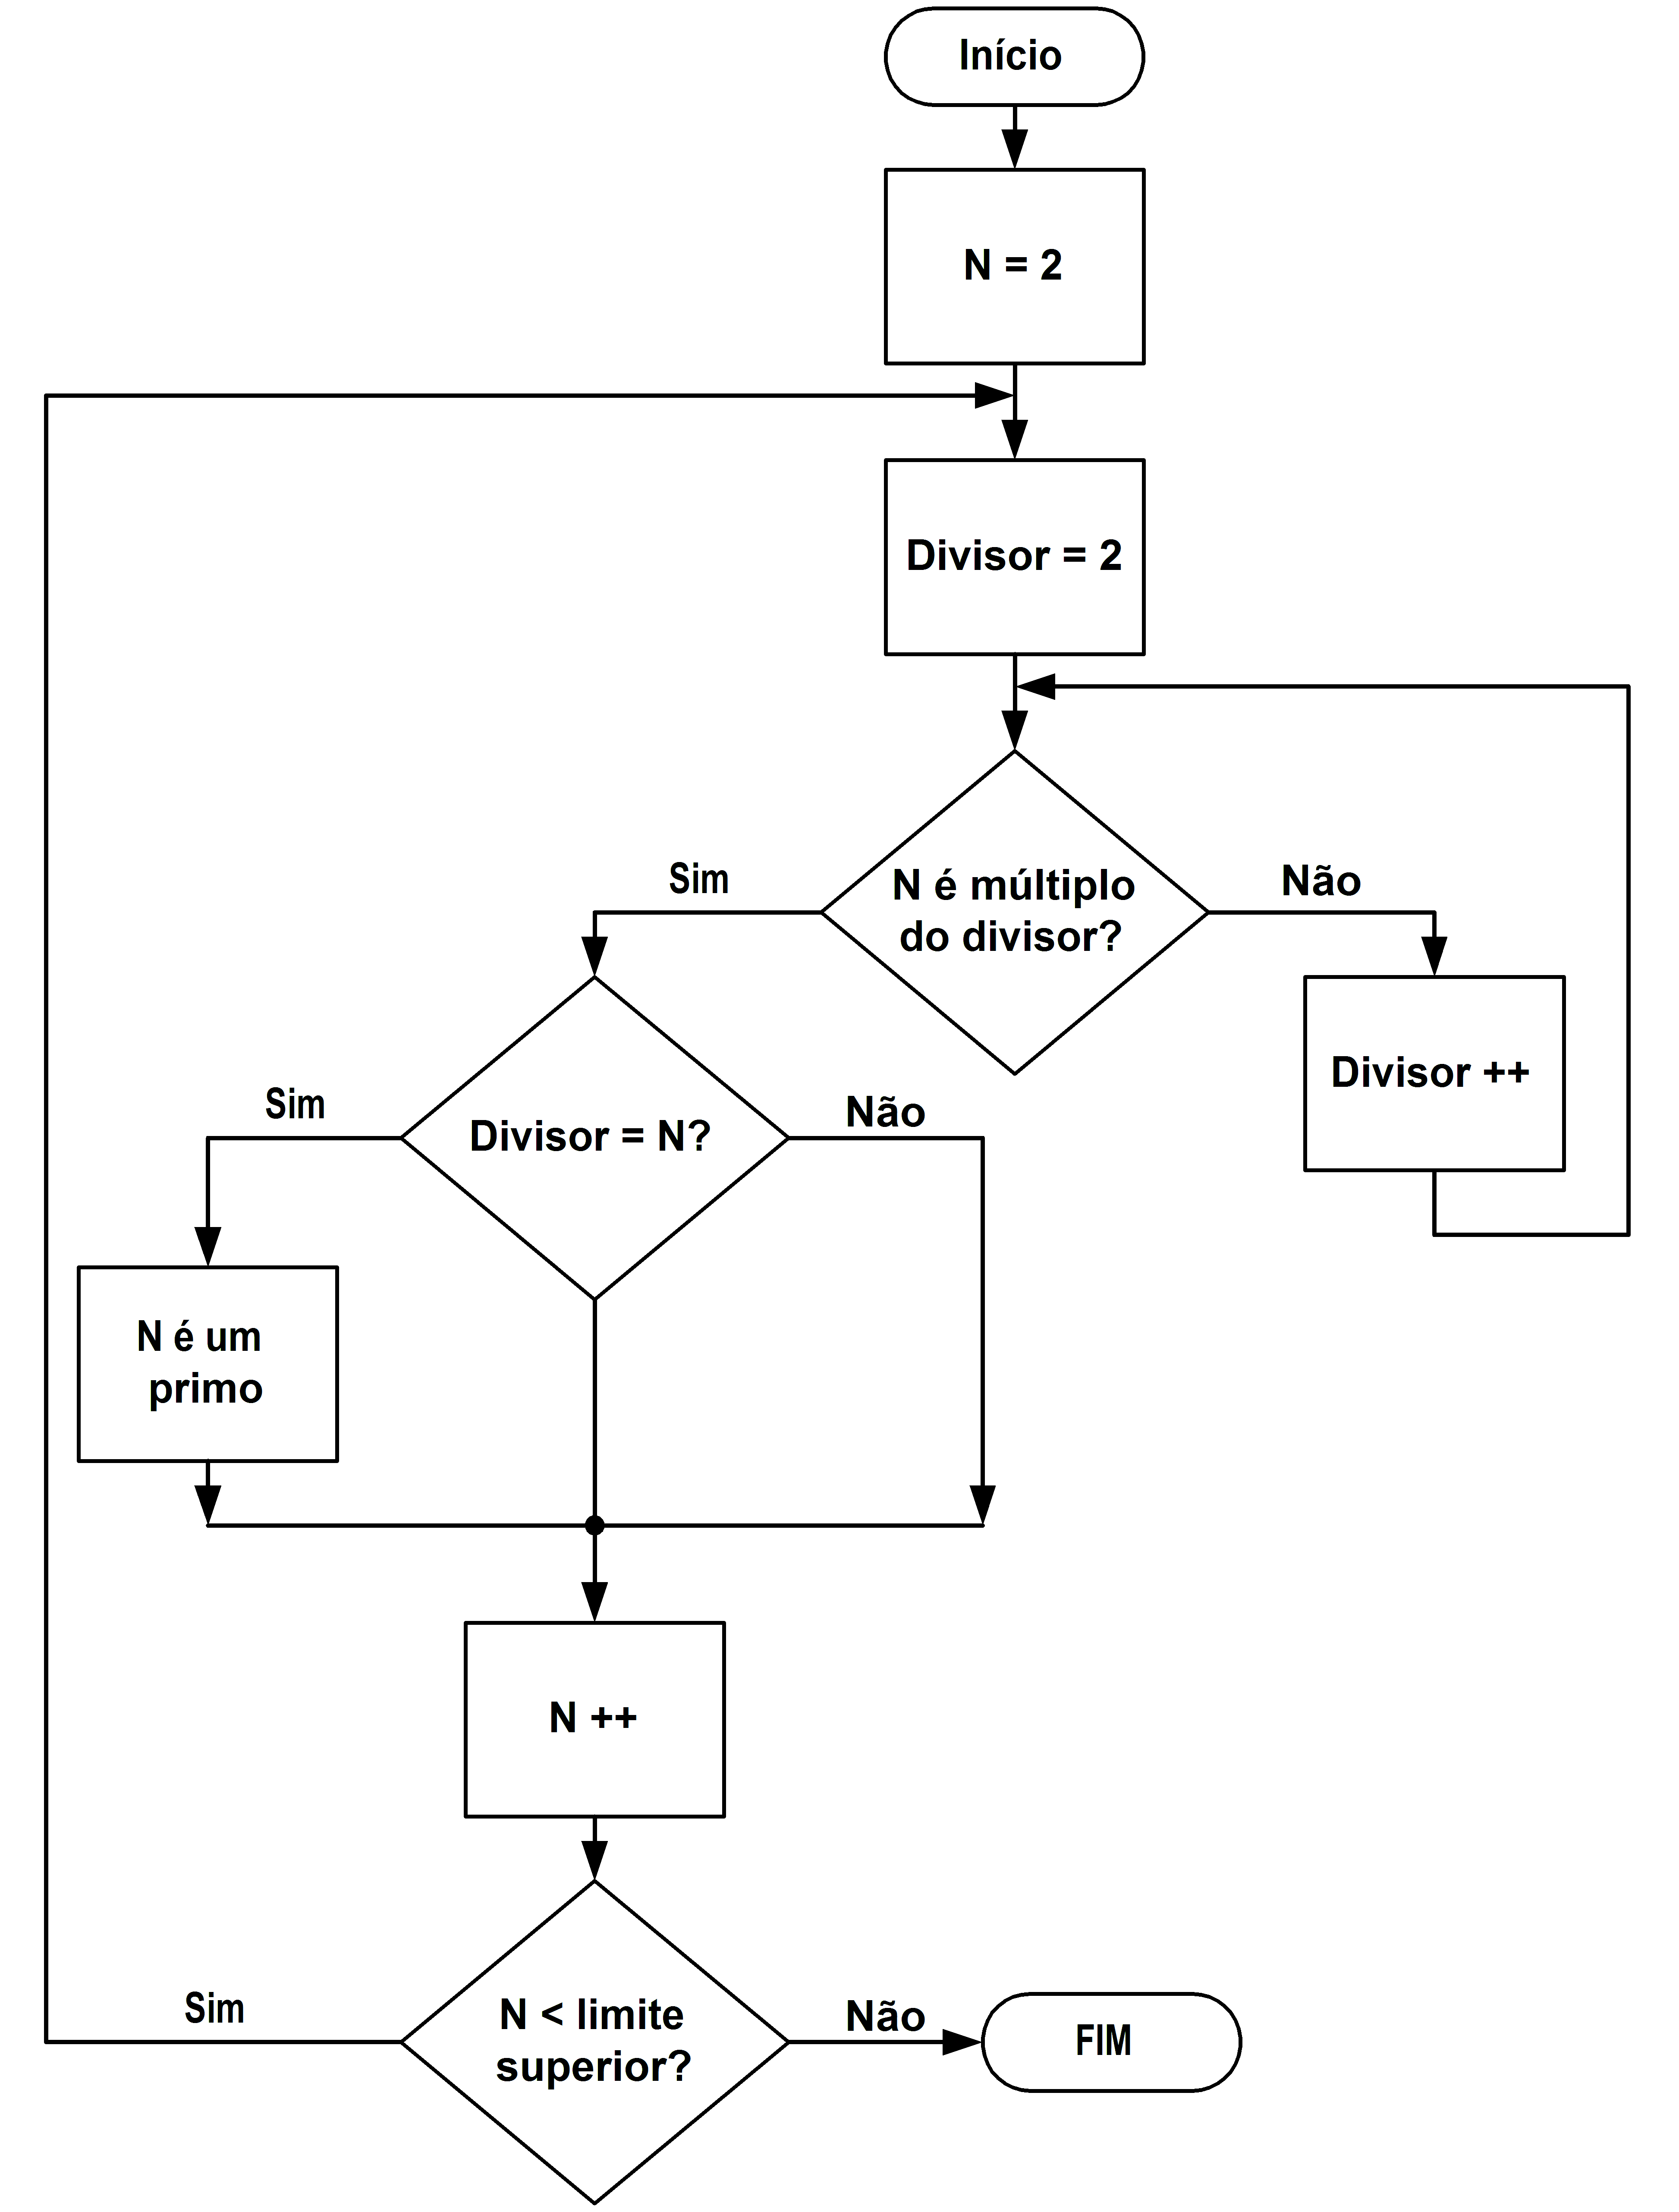
\includegraphics[width=0.5\columnwidth]{Fig1.png}
    \caption{Fluxograma representando a rotina desenvolvida no.....}    
    \label{Instru1}
\end{figure}

\subsection{Sub-capítulo}

Texto Principal.

Texto Principal.

\subsection{Sub-capítulo}

Texto Principal.

Texto Principal.

\section{Resultados e Discussões}

Texto principal.

Texto principal. Aqui devem ser apresentados todos os resultados do trabalho/experimento contendo tabelas, gráficos (figuras) e demais figuras necessárias à compreensão do trabalho/experimento. Todos os conceitos da área de instrumentação devem ser apresentados para cada sistema, como por exemplo, cadeia de medição, resolução, sensibilidade, erro de linearidade, erro de conformidade, etc...

Resumidamente este capítulo deve apresentar os resultados e discussões do que foi feito no capítulo anterior. Jamais uma figura ou tabela deve ficar “solta” no trabalho e a mesma deve ser chamada no texto e conter uma discussão coerente em relação à mesma. É desnecessário afirmar que figuras, tabelas e etc devem ser legíveis para a completa compreensão do texto. Uma boa forma para verificar a qualidade de um texto é deixar outra pessoa ler com atenção seu texto e verificar se a mesma compreendeu o texto! Além disso, sugiro a leitura várias vezes do relatório pelo grupo antes da sua entrega. Os resultados devem ser discutidos baseados nos conceitos de instrumentação – apresentar análise coerente dos dados (usando estatística, análise da propagação de incertezas, etc).

\subsection{Sub-capítulo}

Texto principal.

Texto principal.

Texto principal. Observe que todo e qualquer texto, figura(s), tabela(s) que não sejam originais dos autores devem obrigatoriamente ser apresentadas as correspondentes fontes (o mesmo vale para texto de outros autores). Devemos respeitar os direitos autorais para evitar possíveis problemas de ordem legal e penalidades em função disso. Por exemplo:

\qquad Segundo Balbinot (2010), (citação quando o texto é de apenas um autor) texto texto texto. De acordo com Balbinot  Brusamarello (2011), texto texto texto (citação quando o texto é de dois autores). Para mais de dois autores usar et al., por exemplo, Doebelin et al. (1996), texto texto....


\begin{table}[h]
    \centering
    \caption{Adicionar a legenda da tabela aqui.}
    \label{Tab1}
    \begin{tabular}{ c }
    [adicionar a tabela aqui; usar um gerador de tabelas, por exemplo do MS Word.\\
    Não esquecer de retirar o colchetes no final.]\\
    \end{tabular}
    \source{Sobrenome, 2010 ou Sobreno1 \& Sobrenome2, 2005 ou Sobrenome \textit{et al.}, 1998.}
\end{table}

% Exemplo de Tabela
%\begin{table}[h]
%    \centering
%    \caption{Exemplo de tabela inserida em uma coluna}
%    \label{Tab1}
%    \begin{tabular}{ c c c }
%    \hline
%    \hline
%    $z$ & $r_{\text{rms}}$ & $\varepsilon_{\text{rms}}$ \\ \hline
%    0   & 0,85 & 0    \\
%    50  & 1,65 & 0,82 \\
%    100 & 1,51 & 1,22 \\
%    \hline
%    \hline
%    \end{tabular}
%    \source{Sobrenome, 2010 ou Sobreno1 \& Sobrenome2, 2005 ou Sobrenome \textit{et al.}, 1998.}
%\end{table}

\begin{figure}[H]
    \centering
    [adicionar a figura aqui. Não esquecer de retirar o colchetes no final. Se a figura não foi desenvolvida por vocês citar a fonte. Mesmo quando a figura foi alterada devemos citar que a mesma pertence ao autor original e foi adaptada livremente pelos autores do relatório. Obrigatoriamente toda e qualquer citação deve estar completa nas referência bibliográficas do relatório para consulta dos leitores.]
    \caption{Adicionar uma legenda da figura aqui.}
    \label{Instru1}
    \source{Sobrenome, 2010 ou Sobreno1 \& Sobrenome2, 2005 ou Sobrenome \textit{et al.}, 1998.}
\end{figure}

% Exemplo de Figura
%\begin{figure}[H]
%    \centering
%    \includegraphics[width=0.5\columnwidth]{Instru1.png}
%    \caption{Fluxograma representando a rotina desenvolvida no.....}    
%    \label{Instru1}
%    \source{Sobrenome, 2010 ou Sobreno1 \& Sobrenome2, 2005 ou Sobrenome \textit{et al.}, 1998.}
%\end{figure}

\section{Conclusões}

Texto.

Texto. Quais as conclusões baseada nos seus resultados. Relembrando no capítulo de cetodologia explicaram como “foi feito o experimento”, no capítulo de resultados e discussões explicaram e apresentaram os resultados e discussões do que foi “feito” no capítulo anterior e agora apresentam uma conclusão final sobre o trabalho. Evitar textos do tipo: o trabalho foi válido, aprendemos bastante sobre o conteúdo....isso não é conclusão de um relatório científico! Conclusões sobre o trabalho experimental apenas! Sugiro que façam perguntas para os professores da disciplina e até mostrar com antecedência um dos relatórios.

\section*{Agradecimentos}

Texto.

Texto. Opcional e se necessário. Normalmente usado para agradecer bolsas, verbas de órgãos de fomento e voluntários nos ensaios ou entidades que auxiliaram no trabalho. Não agradecer aos professores pelo aprendizado, pelo trabalho.....isso nem pensar. Agradecimentos com um formato profissional, ou seja, apenas aos órgãos de fomento (que não é o caso aqui), voluntários nos ensaios ou entidades que auxiliaram no trabalho.

\begin{thebibliography}{9}

\setlength{\parskip}{0pt}
\setlength{\itemsep}{0pt plus 0.3ex}
  
\bibitem{sobrenome} 
Sobrenome, A.B.; Sobrenome, C.D. Title of the cited article. \textit{Journal Title} \textbf{2007}, \textit{6}, 100-110.
\bibitem{balbinot} 
Balbinot, A.; Brusamarello, V.J.. Title of the cited article. \textit{Journal Title} \textbf{2007}, \textit{6}, 100-110.
\bibitem{author} 
Author, A.; Author, B. Title of the chapter. \textit{In Book Title}, 2nd ed.; Editor, A., Editor, B., Eds.; Publisher: Publisher Location, Country, 2007; Volume 3, pp. 154-196.pp. 154-196.
\bibitem{author2} 
Author, A.; Author, B. \textit{Book Title}, 3rd ed.; Publisher: Publisher Location, Country, 2008; 
pp. 154-196.
\bibitem{reference} 
Reference list. We recommend the use of reference management software to prepare the references list (e.g. Endnote, http://www.endnote.com/).

\end{thebibliography}

\noindent \copyright \the\ano \ dos autores; disciplina de Instrumentação A, UFRGS, DELET, RS, Brasil. 

\end{document}